\documentclass[tikz]{standalone}
\begin{document}
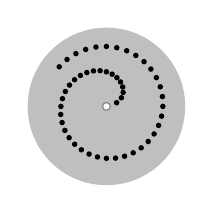
\begin{tikzpicture}
\newcount\myangle
\newcount\myradiusinverse
\fill[gray!50] (0,0) circle (1cm);
\foreach \i in {1,...,50}{
	\myangle=\i
	\multiply\myangle by 10
	\myradiusinverse=\i
	\fill[black] ({(.2*ln(\myradiusinverse)*cos(\myangle)},{.2*ln(\myradiusinverse)*sin(\myangle)}) circle (1pt);
}
\fill[white,draw=gray] (0,0) circle (1.4pt);
\end{tikzpicture}
\end{document}
